\documentclass[12pt,a4paper]{standalone}
\usepackage{amssymb}
\usepackage{amsmath}
\usepackage{bm}
\usepackage{tikz}
\usetikzlibrary{arrows.meta}
\usetikzlibrary{arrows}
\usepackage{pstricks}
\usetikzlibrary{patterns}
\usetikzlibrary{fadings}
\usetikzlibrary{shapes.geometric}







\begin{document}
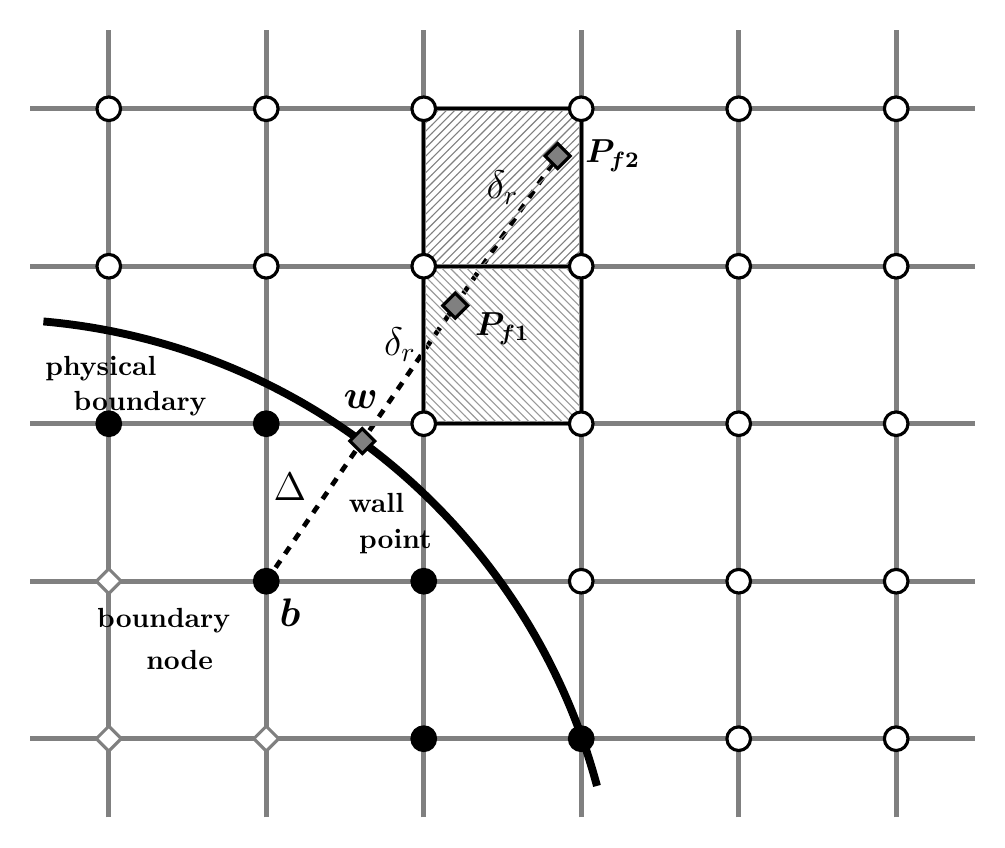
\begin{tikzpicture}[line width=0.4mm]
\draw[dashed,thick,line width=0.6mm] (4,2) -- (7.7,7.4);

\draw[gray,solid,thick,line width=0.6mm] (1,0) -- (13,0);
\draw[gray,solid,thick,line width=0.6mm] (1,2) -- (13,2);
\draw[gray,solid,thick,line width=0.6mm] (1,4) -- (13,4);
\draw[gray,solid,thick,line width=0.6mm] (1,6) -- (13,6);
\draw[gray,solid,thick,line width=0.6mm] (1,8) -- (13,8);

\draw[gray,solid,thick,line width=0.6mm] (2,-1) -- (2,9);
\draw[gray,solid,thick,line width=0.6mm] (4,-1) -- (4,9);
\draw[gray,solid,thick,line width=0.6mm] (6,-1) -- (6,9);
\draw[gray,solid,thick,line width=0.6mm] (8,-1) -- (8,9);
\draw[gray,solid,thick,line width=0.6mm] (10,-1) -- (10,9);
\draw[gray,solid,thick,line width=0.6mm] (12,-1) -- (12,9);

\draw[thick,line width=1mm] (8.2,-0.6) arc[start angle=15, end angle=85, radius=8];
\draw[pattern=north west lines, pattern color=gray!80] (6,4) rectangle (8,6);
\draw[pattern=north east lines, pattern color=gray] (6,6) rectangle (8,8);

%top first row
\draw[black,fill=white] (2,8)node[]{} circle(0.15cm);
\draw[black,fill=white] (4,8)node[]{} circle(0.15cm);
\draw[black,fill=white] (6,8)node[]{} circle(0.15cm);
\draw[black,fill=white] (8,8)node[]{} circle(0.15cm);
\draw[black,fill=white] (10,8)node[]{} circle(0.15cm);
\draw[black,fill=white] (12,8)node[]{} circle(0.15cm);

%top second row
\draw[black,fill=white] (2,6)node[]{} circle(0.15cm);
\draw[black,fill=white] (4,6)node[]{} circle(0.15cm);
\draw[black,fill=white] (6,6)node[]{} circle(0.15cm);
\draw[black,fill=white] (8,6)node[]{} circle(0.15cm);
\draw[black,fill=white] (10,6)node[]{} circle(0.15cm);
\draw[black,fill=white] (12,6)node[]{} circle(0.15cm);

%top third row
\draw[black,fill=black] (2,4)node[]{} circle(0.15cm);
\draw[black,fill=black] (4,4)node[]{} circle(0.15cm);
\draw[black,fill=white] (6,4)node[]{} circle(0.15cm);
\draw[black,fill=white] (8,4)node[]{} circle(0.15cm);
\draw[black,fill=white] (10,4)node[]{} circle(0.15cm);
\draw[black,fill=white] (12,4)node[]{} circle(0.15cm);

%top fourth row
\node [draw, gray, fill=white,diamond, aspect=1,scale=0.7] at (2,2) {};
\draw[black,fill=black] (4,2)node[]{} circle(0.15cm);
\draw[black,fill=black] (6,2)node[]{} circle(0.15cm);
\draw[black,fill=white] (8,2)node[]{} circle(0.15cm);
\draw[black,fill=white] (10,2)node[]{} circle(0.15cm);
\draw[black,fill=white] (12,2)node[]{} circle(0.15cm);

%top fifth row
\node [draw, gray, fill=white,diamond, aspect=1,scale=0.7] at (2,0) {};
\node [draw, gray, fill=white,diamond, aspect=1,scale=0.7] at (4,0) {};
\draw[black,fill=black] (6,0)node[]{} circle(0.15cm);
\draw[black,fill=black] (8,0)node[]{} circle(0.15cm);
\draw[black,fill=white] (10,0)node[]{} circle(0.15cm);
\draw[black,fill=white] (12,0)node[]{} circle(0.15cm);

\node [draw, fill=gray,diamond, aspect=1,scale=0.7] at (5.22,3.78) {};
\node [draw, fill=gray,diamond, aspect=1,scale=0.7] at (6.4,5.5) {};
\node [draw, fill=gray,diamond, aspect=1,scale=0.7] at (7.7,7.4) {};

\draw (7,5.2)node[]{\large{$\bm{P_{f1}}$}};
\draw (8.4,7.4)node[]{\large{$\bm{P_{f2}}$}};


\draw (5.7,5)node[]{\Large{$\delta_r$}};
\draw (7,7)node[]{\Large{$\delta_r$}};
\draw (4.3,3.2)node[]{\Large{$\Delta$}};


\draw (4.3,1.6)node[]{\Large{$\bm{b}$}};
\draw (2.7,1.5)node[]{{\textbf{boundary}}};
\draw (2.9,1)node[]{\textbf{node}};

% \draw (5.8,4.3)node[]{\large{$\bm{f}$}};
% \draw (6.8,3.6)node[]{\textbf{fluid}};
% \draw (6.8,3.1)node[]{\textbf{node}};


% \draw (7.6,6.3)node[]{\large{$\bm{ff}$}};

\draw (5.2,4.3)node[]{\Large{$\bm{w}$}};
\draw (5.4,3)node[]{{\textbf{wall}}};
\draw (5.64,2.5)node[]{{\textbf{point}}};

\draw (1.9,4.7)node[]{{\textbf{physical}}};
\draw (2.4,4.25)node[]{{\textbf{boundary}}};

\end{tikzpicture}



\end{document}



